\documentclass{beamer}
\usepackage{lmodern} %Zorgt voor dat juiste lettergrootte is toegestaan
\usepackage[english]{babel}
\usepackage{graphicx}
\usepackage{amsmath}
\usepackage{amsfonts}
\usepackage{amssymb}
\usepackage{amsthm}
\usepackage{amsfonts}
\usepackage{bbm}
\usepackage{geometry}
\usepackage{tikz}
\usetikzlibrary{positioning,arrows}

\usetheme{Frankfurt}
%\usecolortheme{rose}
%\usecolortheme{seahorse}
\usefonttheme[onlysmall]{structurebold}
\usefonttheme{professionalfonts}
\setbeamercovered{transparent} %Zorgt voor grijze tekst als die nog niet op de slide komt.

\theoremstyle{plain}
\newtheorem{proposition}[theorem]{Proposition}
\newtheorem{property}[theorem]{Property}
\newtheorem{conjecture}[theorem]{Conjecture}

\theoremstyle{definition}
\newtheorem{exercise}[theorem]{Exercise}

\theoremstyle{remark}
\newtheorem{remark}[theorem]{Remark}

\newcommand{\N}{\mathbb{N}}
\newcommand{\R}{\mathbb{R}}
\renewcommand{\P}{\mathbb{P}}
\newcommand{\E}{\mathbb{E}}
\newcommand{\V}{\mathbb{V}}
\newcommand{\1}{\mathbbm{1}}

\title{Paradoxes in probability theory}
\author{Mathijs Kolkhuis Tanke}
\institute{De Leidsche Flesch}
\date{March 20, 2019}

\begin{document}
\begin{frame}
	\titlepage
\end{frame}

\begin{frame} %Met deze commando begin je nieuwe slide
	\frametitle{Table of contents} %Titel van slide
	\tableofcontents 
\end{frame}

\section{Monty Hall's problem}
\subsection*{Introduction}
\begin{frame}
\frametitle{The problem}
\begin{exampleblock}{Monty Hall's game}
\begin{itemize}
\item There are three doors called $a$, $b$ or $c$. One has a car, the others have a goat.
\item Player chooses a door. Without loss of generality choose $a$.
\item Game master opens one of the remaining doors. That door has a goat.
\item Player is asked to switch to the other unopened door.
\item Player wins contents of the door he ultimately chooses.
\end{itemize}
\end{exampleblock}

What is the probability of the other door having a car?
\end{frame}

\begin{frame}
\frametitle{Early `solutions'}
What is the probability of the other door having a car?

\begin{columns}
\column{0.5\linewidth}
\begin{block}{Answer is $\frac{1}{2}$:}
\begin{itemize}
\item There are two doors when the player can switch.
\item One has a car, the other not.
\item The other door has $\frac{1}{2}$ chance of having a car.
\end{itemize}
\end{block}\pause
\column{0.5\linewidth}
\begin{block}{Answer is $\frac{2}{3}$:}
\begin{itemize}
\item Chance of doors $b$ and $c$ having a car is $\frac{2}{3}$.
\item One of them is opened.
\item Thus the other door has chance~$\frac{2}{3}$ of having a car.
\end{itemize}
\end{block}
\end{columns}\pause
\vspace{1em}
In fact, both are wrong. Probability ranges from $\frac{1}{2}$ to $1$.
\end{frame}
\subsection*{Sigma-algebra}
\begin{frame}
\frametitle{Probability spaces}
\begin{definition}[$\sigma$-algebra]
Let $\Omega$ be a set and $\mathcal{P}(\Omega)$ its power set.

The set $\Sigma\subseteq\mathcal{P}(\Omega)$ is a \emph{$\sigma$-algebra} iff
\begin{enumerate}
	\item $\Omega\in\Sigma$,
	\item $\Sigma$ is closed under countable unions,
	\item $\Sigma$ is closed under countable intersections and
	\item $\Sigma$ is closed under complement.
\end{enumerate}
\end{definition}
\pause
\begin{definition}[Probability space]
Let $\Omega$ be a set and $\Sigma$ a $\sigma$-algebra on $\Omega$. Let $\P$ be a probability measure on $\Sigma$.

Then $(\Omega,\Sigma,\P)$ is a probability space.
\end{definition}
\end{frame}

\begin{frame}
\frametitle{Conditional expectation}
We need to extend $\P[A|B]=\frac{\P[A\cap B]}{\P[B]}$.\pause
\begin{definition}[Conditional expectation]
Let $(\Omega,\Sigma,\P)$ be a probability space.

Let $\Sigma'\subseteq\Sigma$ be a sub-$\sigma$-algebra of $\Sigma$.

The \emph{expectation value of $X$ conditioned on $\Sigma'$} is $Y=\E[X|\Sigma']$ s.t.
\begin{itemize}
	\item $Y$ is $\Sigma'$-measurable,
	\item $\E[|Y|]$ is finite and
	\item $\int_A Yd\P=\int_A Xd\P$ for all $A\in\Sigma'$.
\end{itemize}
\end{definition}\pause

\begin{definition}[Conditional probability]
The \emph{probability of $A$ conditioned on $\Sigma'$} is $\P[A|\Sigma']=\E[\1_A|\Sigma']$.
\end{definition}
\end{frame}

\begin{frame}
\frametitle{Back to Monty Hall}
The situation:
\begin{itemize}
	\item $\mathcal{X}=\{a,b,c\}$ is set of doors player can choose.
	\item Take $\Omega=\mathcal{X}$.
	\item $\sigma$-algebra is $\mathcal{P}(\Omega)$.
	\item Condition on smallest $\sigma$-algebra having $\{a,b\}$ and $\{a,c\}$.
\end{itemize}
\pause

However, $\sigma(\{a,b\},\{a,c\})=\mathcal{P}(\Omega)$ is original $\sigma$-algebra.

No information is gained using this conditioning!
\end{frame}

\begin{frame}
\frametitle{Extending the set of possibilities}
The situation:
\begin{itemize}
	\item $\mathcal{X}=\{a,b,c\}$ is set of doors player can choose.
	\item $\mathcal{Y}=\{b,c\}$ is set of doors Monty Hall can open.
	\item Take $\Omega=\mathcal{X}\times\mathcal{Y}$.
	\item $\sigma$-algebra is $\mathcal{P}(\Omega)$.
	\item $X$: r.v.~on $\mathcal{X}$ player choosing a door.
	\item $Y$: r.v.~on $\mathcal{Y}$ which door to open after player's choice.
\end{itemize}
\pause

Then
\begin{align*}
\P[X=a|Y=b]&=\frac{\P[X=a,Y=b]}{\P[Y=b]}\\
&=\frac{\P[X=a,Y=b]}{\sum_{x\in \mathcal{X}}\P[Y=b|X=x]\P[X=x]}.
\end{align*}

$\P[X=x]$ is unknown, thus the conditional probability cannot be calculated. Real answer has many variables.
\end{frame}

\begin{frame}
\frametitle{Example}

\begin{exampleblock}{Probability $\frac{1}{2}$}
If
\begin{itemize}
\item the car is distributed uniformly between the doors,
\item door $a$ is first chosen, 
\item door $a$ actually has the car and
\item Monty Hall never opens door $b$ in this case,
\end{itemize}
then probability of having the correct door is $\frac{1}{2}$.
\end{exampleblock}
\end{frame}

\section{Borel-Kolmogorov paradox}
\subsection*{The situation}
\begin{frame}
\frametitle{The Borel-Kolmogorov paradox}

\begin{exampleblock}{The setting of the Borel-Kolmogorov paradox}
\begin{itemize}
	\item Take a sphere and distribute points uniformly.
	\item Draw a great circle through one point.
	\item Mask all distributed points.
\end{itemize}
\end{exampleblock}
What is the distribution of the point being on the great circle?

\pause

Answer: depends on parametrizations.
\end{frame}

\begin{frame}
\frametitle{Bayesian probability}

Let $C$ be the great circle and $E\subset C$ a subset. Then
\[\P[E|C]=\frac{\P[E\cap C]}{\P[C]}=\frac{0}{0}.\]

The conditional probability is undefined!
\end{frame}

\begin{frame}
\frametitle{Widening our view}

Let $S=[0,2\pi]\times[0,\pi]$ be the unit sphere with spherical coordinates.

The uniform probability measure on $A\subseteq S$ is given by
\[\P[A]=\frac{1}{4\pi}\iint_A \sin\psi d\phi d\psi.\]
\end{frame}

\begin{frame}
\frametitle{Look at longitudes}
The $\sigma$-algebra of longitudes is 
\[\mathfrak{C}=\left\{[0,2\pi]\times A|A\subseteq[0,\pi]\text{ is measurable}\right\}.\]
The conditional expectation on $\mathfrak{C}$ is
\[\E[X|\mathfrak{C}](\phi,\psi)=\frac{1}{2\pi}\int_0^{2\pi}X(\phi',\psi)d\phi'.\]
\pause

The conditional probability of $B=[\phi_1,\phi_2]\times\{\psi'\}$ on $[0,2\pi]\times\{\psi'\}$ is
\[\bar{\P}[B]=\frac{\phi_2-\phi_1}{2\pi},\]
thus the conditional probability stays uniform! 
\end{frame}

\begin{frame}
\frametitle{Look at meridians}
The $\sigma$-algebra of meridians is 
\[\mathfrak{M}=\left\{A\times [0,\pi]|A\subseteq[0,2\pi]\text{ is measurable}\right\}.\]
The conditional expectation on $\mathfrak{M}$ is
\[\E[X|\mathfrak{M}](\phi,\psi)=\frac{1}{2}\int_0^{\pi}X(\phi,\psi')\sin\psi'd\psi'.\]
\pause

The conditional probability of $B=\{\phi'\}\times[\psi_1,\psi_2]$ on $\{\phi'\}\times[0,\pi]$ is
\[\bar{\P}[B]=\frac{1}{2}(\cos\psi_1-\cos\psi_2),\]
thus the conditional probability does not stay uniform! 
\end{frame}

\subsection*{Solution}
\begin{frame}
\frametitle{Recap}

\begin{itemize}
\item Looking at longitudes the conditional distribution is uniform.
\item Looking at meridians the conditional distribution is cosine.
\end{itemize}

Which one is right?
\end{frame}

\begin{frame}
\begin{theorem}[Gyenis, Hofer-Szabó, Rédei (2017)]
Consider probability spaces $(S,\mathfrak{C},\P)$ and $(S,\mathfrak{M},\P)$, then those spaces are not isomorphic.
\end{theorem}\pause
\begin{proof}
\begin{itemize}
	\item Let $f\colon S\to S$ any measurable isomorphism.
	\item Let $h_f\colon\mathfrak{C}\to\mathfrak{M}$ be a Boolean algebra preserving bijection.
	\item If $C$ is longitude, $h_f(C)$ is a meridian.
	\item All meridians cross in $m_0$, set of north and south poles.
	\item Let $c_0$ such that $h_f(c_0)=m_0$. Note that $c_0$ are longitudes.
	\item Then
	\[\emptyset=h_f(\emptyset)=h_f(C\cap c_0)=h_f(C)\cap h_f(c_0)=h_f(C)\cap m_0=m_0.\]
\end{itemize}
\end{proof}
\end{frame}

\begin{frame}
\frametitle{Discussion}
Our two probability spaces are vastly different! So what now?

\begin{figure}[b]
\begin{center}
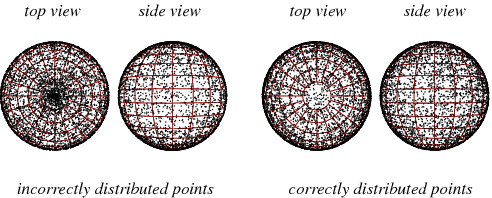
\includegraphics[width=0.6\linewidth]{SphericalDistribution_900.png}
\end{center}
\caption{Simulation by Eric Weisstein}
\end{figure}

\begin{itemize}
	\item Simulate the uniform distribution on the sphere by longitudes and meridians.
	\item If points are placed uniformly on longitudes or cosinely on meridians, the uniform distribution on the sphere is recovered!
\end{itemize}
\end{frame}
\begin{frame}
\frametitle{Asking the right question}
The question
\begin{alertblock}{}
`what is the conditional distribution on the zero set given I have points there'
\end{alertblock}
is unanswerable.
\vspace{1em}

The question for conditional probability must rather be:
\begin{exampleblock}{}
`if I want to simulate the original distribution using this parametrization, what should my conditional probability be?'
\end{exampleblock}
\end{frame}
\section{Two envelope problem}
\begin{frame}
\frametitle{The game}

\begin{exampleblock}{Two envelope game}
\begin{itemize}
	\item Game master picks a value $x$.
	\item Game master fills one envelope with $x$, other with $2x$.
	\item Game master gives an arbitrary envelope to the player.
	\item Player sees contents of his envelope.
	\item Player gets the option to switch to the other envelope.
	\item Should the player switch?
\end{itemize}
\end{exampleblock}
\pause
Call the player's envelope $A$, then
\[\E[B]=\frac{1}{2}\cdot \frac{x}{2}+\frac{1}{2}\cdot 2x=\frac{5}{4}x.\]
Player must always switch!

\end{frame}

\begin{frame}
\frametitle{Playing the game}

Can I get two volunteers?
\end{frame}

\begin{frame}
\frametitle{Probability space}
Probability space:
\begin{itemize}
	\item $\mathcal{X}=\{(x,2x),(2x,x)\}$,
	\item $\Sigma=\mathcal{P}(\mathcal{X})$,
	\item $\P$ is uniform.
\end{itemize}

Then 
\begin{align*}
\E[B]&=\E[B|A=x]\P[A=x]+\E[B|A=2x]\P[A=2x]\\
&=\frac{1}{2}\cdot2x+\frac{1}{2}x=\frac{3}{2}x.
\end{align*}
\pause
Thus $\E[A]=\E[B]=\frac{3}{2}x$, switching does not help!

However, the player does not know $x$...
\end{frame}

\subsection*{Priors}
\begin{frame}
\frametitle{Prior on lowest value}
Let $X$ be the continuous r.v.~for the lowest value $x$ in the envelopes with density $f$.
\begin{itemize}
	\item If $\P[B=2a|A=a]=\P\left[B=\frac{a}{2}\middle|A=a\right]=\frac{1}{2}$, then $X$ is uniform on an unbounded set. This is not possible.
	\item Suppose $\E[X]<\infty$ to avoid the St.~Petersburg paradox.
\end{itemize}
\end{frame}

\begin{frame}
\frametitle{Switching strategies}
\begin{definition}[Switching strategy]
Let $P\colon(0,\infty)\to[0,1]$ be arbitrary. Then $P$ is a \emph{switching strategy} if the player switches his envelope with probability $P(a)$ after observing $a$ in his envelope.
\end{definition}\pause
\begin{definition}[Gain]
Using switching strategy $P$, the player's \emph{gain} relative to never switching is
\[G=\frac{1}{2}\int_0^\infty xf(x)(P(x)-P(2x))dx.\]
\end{definition}\pause
Never switching has gain $G=0$. If $G>0$, then $P$ is a better strategy than never switching. If $G<0$, then $P$ is a worse strategy than never switching.
\end{frame}
\begin{frame}
\frametitle{Positive gains}
\begin{lemma}
If $P$ is decreasing and strictly decreasing on an interval $I$ with $f(I)>0$, then $G>0$.
\end{lemma}\pause
\begin{example}[Threshold switching]
Let $P(x)=\1_{[0,b]}(x)$, thus always switch if value lower than $b$ is encountered. Then $P$ is decreasing and has non-negative gains.

If $f$ is strictly decreasing, choose $b$ such that $f(2b)=\frac{1}{4}f(b)$. This $P$ is the best switching strategy possible.
\end{example}
\end{frame}
\begin{frame}
\frametitle{Optimize threshold switching}

\begin{theorem}[Egozcue and García (2015)]
Let $X$ be continuous with $\E[X]=\mu$ and $\V[X]=\sigma^2$. Let $m=\mu^2+\sigma^2$. Let $P(x)=\1_{[0,b]}(x)$ be threshold switching.
\begin{enumerate}
	\item The gain has lower bound
	\[G(b)\geq\frac{3+2\sqrt{2}}{b}\left(\frac{3}{2}b\mu-\frac{1}{2}b^2-m\right).\]
	\item If $\mu^2> 8\sigma^2$, then $b^*=\sqrt{2m}$ is optimal with gain 
	\[G(b^*)\geq(3+2\sqrt{2})\left(\frac{3}{2}\mu-\sqrt{2m}\right)>0.\]
\end{enumerate}
\end{theorem}
\end{frame}
\begin{frame}
\frametitle{Trade?}

\begin{itemize}
\item Countdown from 3, tell if you want two switch.
\item Switch when both players agree.
\item After possibly switching reveal the contents of your envelopes.
\end{itemize}
\end{frame}
\end{document}
